\documentclass{beamer}

\usepackage{eecs}

\usepackage[all]{xy}
\usepackage{xmpmulti}
\usepackage{pdfpages}
\usepackage{fancyvrb}

\SaveVerb{bind}+>>=+
\SaveVerb{from}+<-+

%\renewenvironment{Verbatim}{\verbatim}{\endverbatim}
% \begin{Verbatim}[fontsize=\footnotesize]


\title[CS]{Introduction to Computer Science}
\author[Andy Gill]{Dr. Andy Gill}
\institute{Electrical Engineering and Computer Science}
\date{December 1st and 5th}

\begin{document}

\frame{\titlepage}

\begin{frame}
\frametitle{Computer Science}
\Large

In this class, we are going to

\frameskip{}
\begin{itemize}
\item {\bf Learn} what it means to program a computer
\item {\bf Learn} basic programming
\item {\bf Enhance} an existing Program (a simple game)
\item {\bf Program} a bot (give a virtual agent ``smarts'')
\end{itemize}
\frameskip{}

Friday is a lab, in the engineering commons.
\end{frame}


\begin{frame}
\frametitle{First - who is Andy Gill?}
\Large

\begin{itemize}
\item Researcher in the field of programming languages
\item Ph.D.\ from the University of Glasgow
\item Spent 12 years in industry as a compiler engineer and technical lead
\begin{itemize}
\item Worked on a Java compiler, a C++ compiler, and a Haskell compiler 
\item Co-founded a technology startup in Portland, OR, that used Haskell
\end{itemize}
\item Teaching since 2002; moved to KU in 2008.
\item Want to share my research interests: Computers and Programming Languages
\end{itemize}

\end{frame}

\begin{frame}
\frametitle{What is a Computer?}
\large

``The trouble with computers is, they're very sophisticated idiots. They do exactly what you tell them at amazing speeds.'' 

\begin{center}
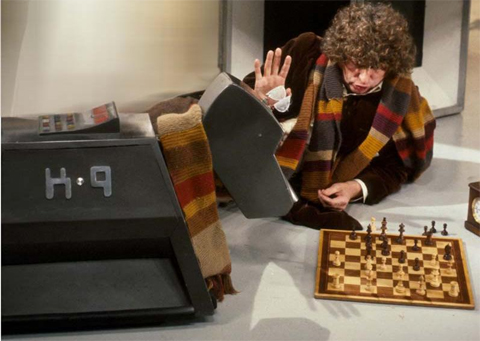
\includegraphics[width=0.4\textwidth]{computersanddoctorwho.jpg}
\end{center}


~~~--- The 4th Doctor.

\end{frame}

\begin{frame}   
\frametitle{Why do we have computers?}
\Large

\begin{center}
\href{file:/Users/andy/git/github/engr108/slides/JobsBike.mov}{?}
\end{center}

\end{frame}

\begin{frame}
\frametitle{Computer Science is {\bf not}}
\Large
Computer Science is {\bf not\/} about programming.
\frameskip

\begin{itemize}
\item CS uses programming as a tool to get a job done.
\item CS uses programming in the same way most engineering subjects use Math.
\item Furthermore, programming is its own type of Math.
\item Programming can be executable and/or declarative.
\end{itemize}

\frameskip
We are going to see some basic programming today.
\end{frame}

\begin{frame}
\frametitle{What does Computer Science using {\bf programming} for?}
\Large
\begin{itemize}
\item Mechanization --- Example: HVAC controller
\item Simulation --- CS helping others
\item Graphics --- User Interfaces
\item Search --- Finding things
\item Storage --- ``The Cloud''
\item The Web --- Online shopping carts
\end{itemize}

All use programming as a means to an end.

\end{frame}

\begin{frame}
\frametitle{What does Computer Science using {\bf programming} for?}
\Large

Think of a single digit number.

\begin{enumerate}
\item Square it.
\item Add the result to your original number.
\item Divide by your original number.
\item Add, oh, how about 17.
\item Subtract your original number.
\item Divide by 6. 
\end{enumerate}

We are going to automate (program) this.

\end{frame}


\begin{frame}[fragile]
\frametitle{Programming ``Think of a number''}

\begin{codeblock}
\begin{verbatim}
// Think of a number.                                                                                                     
x = 9;
// Square it.                                                                                                                  
a = x * x;
// Add the result to your original number.                                                                                     
a = a + x;
// Divide by your original number.                                                                                             
a = a / x;
// Add, oh, how about 17.                                                                                                      
a = a + 17;
// Subtract your original number.                                                                                              
a = a - x;
// Divide by 6.                                                                                                                
a = a / 6;
// Print the number to the screen.
console.log(a);
\end{verbatim}                
\end{codeblock}
\end{frame}

\begin{frame}[fragile]
\frametitle{2nd Problem - find your direction}
\Large

\begin{itemize}
\item You are on a 2-dimensional plane.
\item You want to point towards another (given) point on the plane.
\item How do you compute this?
\end{itemize}

\frameskip

if $x,y$ are your coordinates, then $atan2(y,x)$
is the direction you are from the origin, in radians.

\end{frame}


\begin{frame}[fragile]
\frametitle{Programming ``Find your direction''}

\begin{codeblock}
\begin{verbatim}
// Original Coords.
x = 3; y = 4;

// Target Coords.
xt = 5; yt = 2;

// Take the difference between the vectors.
xd = xt - x;
yd = yt - y;

// Compute the radian                                                                                                         
r = atan2(yd,xd);

// Print the result.
console.log(r);
\end{verbatim}                
\end{codeblock}
\end{frame}

\begin{frame}[fragile]
\frametitle{Types of expressions}
\Large

Expressions are on the right hand side of assignments.

Numbers:
\begin{itemize}
\item {\bf 1, 2, -1, -2, \ldots}
\end{itemize}

Arithmetic:
\begin{itemize}
\item {\bf \verb$+$, \verb$-$, \verb$*$, \verb$/$}
\end{itemize}

Parenthesis:
\begin{itemize}
\item {\bf \verb$($~\ldots~\verb$)$}
\end{itemize}

\end{frame}

\begin{frame}[fragile]
\frametitle{Assignment Statements}
\Large

{\centering{\Huge var = expr ;}}

\frameskip{}
{\bf var} is a variable name. letters and numbers, starting with a letter.
Upper case is for constant variables, like {\bf PI}.
\frameskip{}
{\bf expr} is an expression, like {\bf x + 1}. Complex expressions are allowed,
as are parenthesis. expressions can contain calls to functions, like {\bf atan2}.
\frameskip{}
Remember to close with semi-colon.

\end{frame}

\begin{frame}[fragile]
\frametitle{Controlling the boat}
\Large 
Task: 
\begin{itemize}
\item Make the boat go North.
\item (Get eaten by monster.)
\end{itemize}
\frameskip{}
\frameskip{}
\begin{itemize}
\item Question: Is there a way of escaping?
\end{itemize}

\end{frame}


\begin{frame}[fragile]
\frametitle{What if we want to do something conditionally?}
\Large
Conditionals are a way of making choices.

Task: 
\begin{itemize}
\item Assign {\bf x} to -1,0 or 1, depending if {\bf y} is negative, zero, or positive.
\item Split this problem into three parts first.
\end{itemize}

\end{frame}

\begin{frame}[fragile]
\frametitle{Computing absolutes}
\large

\begin{codeblock}
\begin{verbatim}
y = 0;
if (y < 0) {
    x = -1;
}

if (y == 0) {
    x = 0;
}

if (y > 0) {
    x = 1;
}
console.log(x);
\end{verbatim}
\end{codeblock}

\end{frame}

\begin{frame}[fragile]
\frametitle{Form of a conditional}
\large

{\Huge if (condition) \{}\\
{\Huge ~~~~ assignment; }\\
{\Huge ~~~~ assignment; }\\
{\Huge ~~~~ assignment; }\\
{\Huge \}}
\end{frame}


\begin{frame}[fragile]
\frametitle{Types of conditions}
\large
The boring ones:
\begin{itemize}
\item {\bf true, false}
\end{itemize}

Equality and inequality:
\begin{itemize}
\item {\bf \verb$==$, \verb$!=$}
\end{itemize}

Comparisons:
\begin{itemize}
\item {\bf \verb$<$, \verb$<=$, \verb$>$, \verb$>=$}
\end{itemize}

not!
\begin{itemize}
\item {\bf \verb$!$}
\end{itemize}

Chaining comparisons:
\begin{itemize}
\item {\bf \verb$&&$, \verb$||$}
\end{itemize}

Parenthesis:
\begin{itemize}
\item {\bf \verb$($~\ldots~\verb$)$}
\end{itemize}

\end{frame}

\begin{frame}[fragile]
\frametitle{Aside\ldots}

\begin{itemize}
\item Almost everything in computer science can be nested.
\item {\bf if} statements can contain {\bf if} statements.
\item {\bf if} statements can contain {\bf if} statements that
contain {\bf if} statements.
\item \ldots
\end{itemize}

\end{frame}

\begin{frame}[fragile]
\frametitle{New task}

Control the boat.
\begin{itemize}
\item Make the boat go North.
\item After 100 {\em steps\/}, make the boat go West.
\end{itemize}

\frameskip

Advanced:
\begin{itemize}
\item Make the boat go North.
\item After 100 {\em steps\/}, make the boat turn West {\bf gradually}.
\end{itemize}
\end{frame}


\begin{frame}[fragile]
\frametitle{Assignment Statements and Conditionals}
\Large
\begin{itemize}
\item We have learned about {\bf assignment statements}.
\item Assignments give a new value to a named variable.
\item Assignments compute this new value.
\frameskip
\frameskip{}
\item We have learned about {\bf conditionals}.
\item Conditionals {\em optionally\/} do assignments.
\frameskip{}
\frameskip{}
\item On Monday 
\begin{itemize}
\Large
\item Lab (in Eaton 1014 / 1018)
\item Escape from Crater Lake!
\end{itemize}
\end{itemize}

\end{frame}


\end{document}
